%%%%%%%%%%%%%%%%%%%%%%%%%%%%%%%%%%%%%%%%%
% Memo
% LaTeX Template
% Version 1.0 (30/12/13)
%
% This template has been downloaded from:
% http://www.LaTeXTemplates.com
%
% Original author:
% Rob Oakes (http://www.oak-tree.us) with modifications by:
% Vel (vel@latextemplates.com)
%
% License:
% CC BY-NC-SA 3.0 (http://creativecommons.org/licenses/by-nc-sa/3.0/)
%
%%%%%%%%%%%%%%%%%%%%%%%%%%%%%%%%%%%%%%%%%

\documentclass[letterpaper,11pt]{texMemo} % Set the paper size (letterpaper, a4paper, etc) and font size (10pt, 11pt or 12pt)

\usepackage{fancyhdr}
\usepackage{fancybox}
\usepackage{longtable}
\usepackage{amsmath}
%----------------------------------------------------------------------------------------
%	MEMO INFORMATION
%----------------------------------------------------------------------------------------



\memoto{Luis Andr\'es Valido Fajardo. luis.valido@umcc.cu (53694742)} % Recipient(s)

\memofrom{Josval Díaz Blanco} % Sender(s)

\memosubject{Guía de Aprendizaje para Concursantes ICPC y IOI: Búsqueda Binaria } % Memo subject

\memodate{\today} % Date, set to \today for automatically printing todays date

\logo{
\includegraphics[scale=0.5]{img/icpc}} % Institution logo at the top right of the memo, comment out this line for no logo

%----------------------------------------------------------------------------------------

\titleguide{Los caminos más largos de los nodos de un árbol}%all_longest_paths_tree

\begin{document}

%\AddToShipoutPicture{\BackgroundPic}
\maketitle % Print the memo header information
%\tableofcontents
\pagestyle{plain}
\pagebreak

\pagestyle{fancy}
\fancyhead[LO,CE]{ }
\fancyhead[RO,CE]{
\includegraphics[scale=0.1]{img/icpc}}
\fancyfoot[LO,CE]{\textbf{Autor:} Luis Andrés Valido Fajardo \\ \textbf{Email:} luis.valido1989@gmail.com \\ \textbf{Teléfono:} 53694742}
\fancyfoot[RO,CE]{\emph{Existen 10 tipos de personas Las que \\saben binario y LAS QUE NO}}
\fancypagestyle{plain}{\pagestyle{fancy}}



%\lhead{ }
%\rhead{  }

%\fancyfoot[L]{}
%\fancyfoot[R]{\textbf{Autor:} Luis Andrés Valido Fajardo \\ \textbf{Email:} luis.valido@umcc.cu}
%----------------------------------------------------------------------------------------
%	MEMO CONTENT
%----------------------------------------------------------------------------------------


\section{Introducción}
Digamos que tenemos un árbol y queremos calcular para cada nodo del árbol la longitud máxima de un camino que comienza en ese nodo. Esto puede verse como una generalización del problema del diámetro del árbol, porque la mayor de esas longitudes es igual al diámetro del árbol. 

Como ejemplo, considere el siguiente árbol:

% TODO: \usepackage{graphicx} required
\begin{figure}[h!]
	\centering
	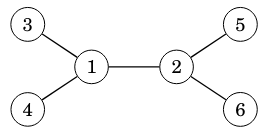
\includegraphics[width=0.4\linewidth]{img/all_longest_paths_1}

	\label{fig:alllongestpaths1}
\end{figure}

Sea $maxLength(x)$ la longitud máxima de una ruta que comienza en el nodo $x$. Por ejemplo, en el árbol anterior, $maxLength(4) = 3$, porque hay una ruta $4 \rightarrow 1 \rightarrow 2 \rightarrow 6$. Aquí hay una tabla completa de los valores:

$$
\begin{array}{r|cccccc}
\text{node x} 	& 1 & 2 & 3 & 4 & 5 & 6 \\
maxLength(x) 	& 2 & 2 & 3 & 3 & 3 & 3
\end{array}
$$

En la presente guía abordaremos como determinar para cada nodo del árbol la longitud máxima de un camino que comienza en ese nodo
\section{Conocimientos previos}
\subsection{Recorrido en Profundidad (\emph{DFS})}
Búsqueda en profundidad. Una Búsqueda en profundidad (en inglés \emph{DFS} o \emph{Depth First Search}) es un algoritmo que permite recorrer todos los nodos de un grafo o árbol (teoría de grafos) de manera ordenada, pero no uniforme. Su funcionamiento consiste en ir expandiendo todos y cada uno de los nodos que va localizando, de forma recurrente, en un camino concreto. Cuando ya no quedan más nodos que visitar en dicho camino, regresa (Backtracking), de modo que repite el mismo proceso con cada uno de los hermanos del nodo ya procesado.
\section{Desarrollo}
La idea trivial de la solución a este ejercicio sería realizar un DFS por cada nodo y para dicho ver al nodo más lejano que puede llegar y este sería el camino maslargo para el nodo por donde se comenzo el DFS. Esta idea el único inconveniente es el alto costo temporal para cuando el árbol tenga gran cantidad de nodos ya que su complejidad temporal esta dada por la expresión O($N(N+E)$) donde $N$ sería la cantidad de nodos del árbol y $E$ las aristas del mismo que por definición de un árbol sería $N-1$ por lo que sustituyen en la expresión inicial nos queda O($2N^2-N$). Pero esta idea del DFS nos va a servir para ver la primera variante de solución.

\subsection{Programación dinámica con DFS}
También en este problema, un buen punto de partida para resolver el problema es rootear el árbol arbitrariamente:
\begin{figure}[h!]
	\centering
	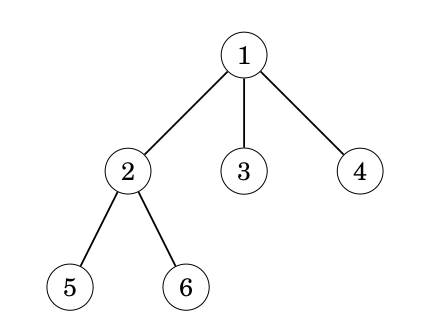
\includegraphics[width=0.4\linewidth]{img/all_longest_paths_2}
	
	\label{fig:alllongestpaths2}
\end{figure}
La primera parte del problema es calcular para cada nodo $x$ la longitud máxima de una ruta que pasa por un hijo de $x$. Por ejemplo, la ruta más larga del nodo $1$ pasa por su hijo $2$:

\begin{figure}[h!]
	\centering
	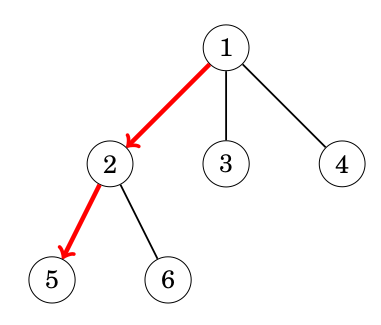
\includegraphics[width=0.4\linewidth]{img/all_longest_paths_3}
	
	\label{fig:alllongestpaths3}
\end{figure}

Esta parte es fácil de resolver en el tiempo O($N$), porque podemos usar la programación dinámica.

Luego, la segunda parte del problema es calcular para cada nodo $x$ la longitud máxima de una ruta a través de su padre $p$. Por ejemplo, la ruta más larga del nodo $3$ pasa por su padre $1$:

\begin{figure}[h!]
	\centering
	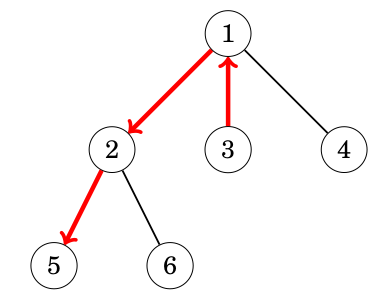
\includegraphics[width=0.4\linewidth]{img/all_longest_paths_4}
	
	\label{fig:alllongestpaths4}
\end{figure}

A primera vista, parece que debemos elegir el camino más largo desde $p$. Sin embargo, esto no siempre funciona, porque el camino más largo de $p$ puede pasar por $x$. Aquí hay un ejemplo de esta situación:

\begin{figure}[h!]
	\centering
	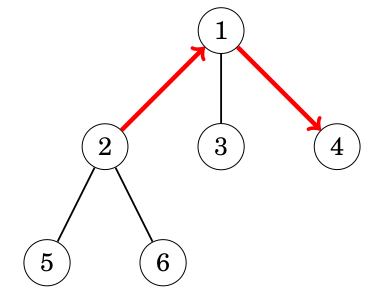
\includegraphics[width=0.4\linewidth]{img/all_longest_paths_5}
	
	\label{fig:alllongestpaths5}
\end{figure}

Aún así, podemos resolver la segunda parte en el tiempo O ($n$) almacenando dos longitudes máximas para cada nodo $x$:

\begin{itemize}
	\item \textbf{$maxLength_1(x)$:} La longitud máxima de una ruta desde $x$
	\item \textbf{$maxLength_2(x)$:} La longitud máxima de una ruta desde $x$ en otra dirección que la primera ruta
\end{itemize}
Por ejemplo, en el anterioranterior, $maxLength_1(1)=2$ usando la ruta $1 \rightarrow 2 \rightarrow 5$, y $maxLength_2(1)=1$ usando la ruta $1 \rightarrow 3$.

Finalmente, si la ruta que corresponde a $maxLength_1(p)$ pasa por $x$, concluimos que la longitud máxima es $maxlength_2(p)+1$, y de lo contrario la longitud máxima es la $maxLength_1(p)+1$.

\subsection{Usando BFS}
Otra idea algorítmica para resolver este problema se basa en la utilización del algoritmo \emph{BFS} con ciertas modificaciones y una estructura como vector o arreglo para almacenar para cada nodo el máximo camino donde él es uno de los extremos.

La idea algorítmica parte del díametro del árbol donde un árbol puede tener uno o varios díametros representados por todos aquellos caminos cuya longitud es máxima en todo el árbol y que comienza en un nodo $u$ y terminan en un nodo $v$. 

Para cualquier nodo $z$ el máximo camino que lo comprende y comienza en él va terminar siempre en un nodo de tipo $u$ o $v$. Por tanto basta con seleccionar un par $(u,v)$ en el árbol y realizar un bfs partiendo sobre cada uno de ellos y ver para cada nodo del árbol de cual de estos dos nodos esta más lejos y ese será el máximo camino para el nodo. Para llevar esta idea vamos a tener dos elementos importantes:

\begin{enumerate}
	\item Un vector o arreglo $path$ con la capacidad igual a la cantidad de nodos con un valor bien pequeño inicialmente. La idea de este vector o arreglo es que voy almacenar en la posición $path[i]$ la longitud máxima de un camino en el árbol donde uno de los extremos de dicho camino es el nodo $i$.
	\item Implementar un \emph{BFS} que retorne el último nodo visitado y que calcule la distancia desde el nodo que se comenzo el \emph{BFS} hacia cualquier otro nodo $i$ del árbol si dicha distancia es mayor que la que se tiene almacenada en el $path$ para el nodo $i$ actualizar el valor de $path[i]$ con dicho valor.
\end{enumerate}

Una vez visto estos detalles el procedimiento sería bien sencillo:

\begin{enumerate}
\item Realizar el \emph{BFS} modificado desde cualquier nodo del árbol escogido de forma arbitraria este nos va devolver un posible nodo $u$.
\item Realizar el \emph{BFS} modificado desde el nodo $u$ obtenido en el paso anterior. Esta ejecucción del \emph{BFS} nos va devolver un posible nodo $v$ asociado con $u$ cuyo camino entre ellos es un diámetro del árbol.
\item Realizar el \emph{BFS} modificado desde el nodo $v$ obtenido en el paso anterior.
 
\end{enumerate}

Una vez realizados estos tres \emph{BFS} en el vector o arreglo $path$ en la posición $i$ tenemos el valor de la longitud del máximo que comienza o termina en el nodo $i$. 


\section{Implementación}
\subsection{C++}

\subsection{Java}
\section{Aplicaciones}
Dentro de las aplicaciones de hallar los caminos más largos de un árbol podemos mencionar:

\begin{enumerate}
	\item \textbf{ Redes de comunicación:} en una red de comunicación, el árbol de ruta más largo se puede utilizar para determinar la ruta más eficiente para transmitir datos o mensajes entre diferentes nodos. Al encontrar el árbol de ruta más largo, los administradores de red pueden optimizar el rendimiento de la red y minimizar los retrasos.
	\item \textbf{Redes de transporte:} los árboles de caminos más largos se pueden aplicar a redes de transporte como carreteras o ferrocarriles. Al identificar los caminos más largos, los planificadores de transporte pueden determinar las rutas más eficientes para vehículos o trenes, reduciendo el tiempo de viaje y la congestión.
	\item  \textbf{Gestión de la cadena de suministro:} en la gestión de la cadena de suministro, se pueden utilizar árboles de ruta más largos para optimizar el flujo de bienes de los proveedores a los clientes. Al identificar los caminos más largos, los gerentes pueden identificar posibles cuellos de botella o ineficiencias en la cadena de suministro y realizar los ajustes necesarios para mejorar la eficiencia general.
	\item \textbf{Gestión de proyectos:} los árboles de ruta más larga se utilizan comúnmente en la gestión de proyectos para determinar la ruta crítica de un proyecto. La ruta crítica es la ruta más larga a través de las actividades de un proyecto, e identificarla ayuda a los gerentes a programar tareas y asignar recursos de manera efectiva para garantizar la finalización oportuna del proyecto.
	\item  \textbf{Análisis de datos:} en el análisis de datos, los árboles de ruta más largos se pueden utilizar para identificar elementos influyentes o importantes dentro de un conjunto de datos. Al encontrar los caminos más largos, los analistas pueden identificar variables o factores clave que tienen el impacto más significativo en el resultado que se analiza.
	\item \textbf{Análisis de redes sociales:} los árboles de ruta más larga se pueden aplicar al análisis de redes sociales para identificar individuos o grupos influyentes dentro de una red. Al encontrar los caminos más largos, los analistas pueden determinar quién tiene más conexiones o influencia dentro de una red social, lo que puede ser útil para estrategias de marketing o para comprender la dinámica social.
	\item \textbf{Investigación genealógica:} en la investigación genealógica, los árboles de caminos más largos se pueden utilizar para rastrear líneas ancestrales y determinar relaciones entre individuos. Al encontrar los caminos más largos, los investigadores pueden identificar ancestros comunes y construir árboles genealógicos.
	\item \textbf{ Enrutamiento de Internet:} los árboles de ruta más largos se utilizan en protocolos de enrutamiento de Internet como el Border Gateway Protocol (BGP) para determinar la mejor ruta para enrutar paquetes de datos entre diferentes redes. Al encontrar las rutas más largas, los enrutadores pueden tomar decisiones informadas sobre las rutas más eficientes para la transmisión de datos.
	\item \textbf{Procesos de toma de decisiones:} los árboles de camino más largo se pueden utilizar en los procesos de toma de decisiones para evaluar múltiples opciones y determinar la opción más favorable u óptima. Al encontrar los caminos más largos, los tomadores de decisiones pueden evaluar los posibles resultados y consecuencias de diferentes opciones y tomar decisiones.
\end{enumerate}

\section{Complejidad}
En  cuanto a la complejidad de los algoritmos analizamos en esta guía podemos mencionar que la primera variante utilizando programación dinámica con dos DFS hace que esta solución tenga una complejidad temporal de  O($2(V+E)$) donde $V$ es la cantidad de vértices del árbol y $E$ las aristas, pero reglas del cálculo de complejidades de algoritmo la constante $2$ se desprecia (en lo personal eso se ve muy bonito para las reglas pero para la programación competitiva es importante tener en cuenta para la cantidad de operaciones), otra sustitución dentro de la expresión es que la cantidad de aristas de un árbol es igual a la cantidad de vértices del árbol por tanto $E = V-1$ y sustituyendo en la expresión final nos queda O($2(2V-1)$).

En cuanto a la complejidad temporal de la segunda variante como se realiza 3 \emph{BFS} la misma es O($3(V+E)$) que haciendo un análisis similar al anterior y sustiyendo $E$ por su equivalente en función de $V$ nos queda O($3(2V-1)$). 

Viendo ya complejidades de ambas variantes algorítmicas es evidente que la basada en programación dinámica es un tanto mas rápida que la basada en \emph{BFS} aunque a favor de esta que su implementación es más facil de implementar y se basa en una idea mas asequible de entender.  
\section{Ejercicios}
A continuación una lista de ejercicios que pueden ser resueltos aplicando los algoritmos analizados en la presente guía:

\begin{itemize}
	\item \href{https://cses.fi/problemset/task/1132/}{CSES - Tree Distances I}
\end{itemize}

\end{document}